\section{Precise Definition of a Limit}\label{sec:LimitsFormal}


This section introduces the formal definition of a limit. Many refer to this as ``the epsilon--delta,'' definition, referring to the letters $\epsilon$ and $\delta$ of the Greek alphabet.\\

Before we give the actual definition, let's consider a few informal ways of describing a limit.  Given a function $y=f(x)$ and an $x$-value, $c$, we say that ``the limit of the function $f$, as $x$ approaches $c$, is a value~$L$'': 

\begin{description}
\item[1.]if ``$y$ tends to $L$'' as ``$x$ tends to $c$.''
\item[2.]if ``$y$ approaches $L$'' as ``$x$ approaches $c$.''
\item[3.]if ``$y$ is near $L$'' whenever ``$x$ is near $c$.''
\end{description}

The problem with these definitions is that the words ``tends,'' ``approach,'' and especially ``near'' are not exact.  In what way does the variable $x$ tend to, or approach, $c$? How near do $x$ and $y$ have to be to $c$ and $L$, respectively?  \\

The definition we describe in this section comes from formalizing {\bf 3}.  A quick restatement gets us closer to what we want:

\begin{description}
\item[$\textbf{3}^\prime$.]If $x$ is within a certain \textit{tolerance level} of $c$, then the corresponding value $y=f(x)$ is within a certain \textit{tolerance level} of $L$.
\end{description}

The traditional notation for the $x$-tolerance is the lowercase Greek letter delta, or $\delta$, and the $y$-tolerance is denoted by lowercase epsilon, or $\epsilon$. One more rephrasing of $\textbf{3}^\prime$ nearly gets us to the actual definition:

\begin{description}
\item[$\textbf{3}^{\prime \prime}$.]If $x$ is within $\delta$ units of $c$, then the corresponding value of $y$ is within $\epsilon$ units of $L$.
\end{description}

We can write ``$x$ is within $\delta$ units of $c$'' mathematically as
$$|x-c| < \delta, \qquad \text{which is equivalent to }\qquad c-\delta < x < c+\delta.$$
Letting the symbol ``$\longrightarrow$'' represent the word ``implies,'' we can rewrite $\textbf{3}''$ as 
$$
|x - c| < \delta \longrightarrow  |y - L| < \epsilon 
\qquad \textrm{or} \qquad c - \delta < x < c + \delta \longrightarrow L - \epsilon < y < L + \epsilon.
$$
The point is that $\delta$ and $\epsilon$, being tolerances, can be any positive (but typically small) values.  Finally, we have the formal definition of the limit with the notation  seen in the previous section.



\begin{definition}{The Limit of a Function $f$}{def:limit}
{Let $I$ be an open interval containing $c$, and let $f$ be a function defined on $I$, except possibly at $c$. The \textit{limit of $f(x)$, as $x$ approaches $c$, is $L$}, denoted by  
$$\displaystyle \lim_{x\rightarrow c} f(x) = L,$$
means that given any $\epsilon > 0$, there exists $\delta > 0$ such that for all $x\neq c$,  
if  $|x - c| < \delta$, then $|f(x) - L| < \epsilon$.\index{limit!definition}
}
\end{definition}


(Mathematicians often enjoy writing ideas without using any words. Here is the wordless definition of the limit:\\

$\displaystyle \lim_{x\rightarrow c} f(x) = L \iff$
$\forall \, \epsilon > 0, \exists \, \delta > 0 \; s.t. \;
0<|x - c| < \delta \longrightarrow |f(x) - L| < \epsilon$.\text{)}\\

Note the order in which $\epsilon$ and $\delta$ are given.  In the definition, the $y$-tolerance $\epsilon$ is given \textit{first} and then the limit will exist {\bf if} we can find an $x$-tolerance $\delta$ that works.  

An example will help us understand this definition.  Note that the explanation is long, but it will take one through all steps necessary to understand the ideas.\\


\begin{example}{Evaluating a limit using the definition}{ex_compute_lim1}{
Show that $\displaystyle \lim_{x\rightarrow 4} \sqrt{x} = 2 $.}
\end{example}


\begin{solution}
{Before we use the formal definition, let's try some numerical tolerances.  What if the $y$ tolerance is 0.5, or $\epsilon =0.5$?  How close to 4 does $x$ have to be so that $y$ is within 0.5 units of 2, i.e., $1.5 < y < 2.5$?  In this case, we can proceed as follows:
\begin{align*}
1.5 &< \parbox{15pt}{\centering $y$} < 2.5 \\
1.5 &< \parbox{15pt}{\centering $\sqrt{x}$} < 2.5\\
1.5^2 &< \parbox{15pt}{\centering $x$} < 2.5^2\\
2.25 &< \parbox{15pt}{\centering $x$} < 6.25.
\end{align*}

So, what is the desired $x$ tolerance?  Remember, we want to find a symmetric interval of $x$ values, namely
$4 - \delta < x < 4 + \delta$.  The lower bound of $2.25$ is $1.75$ units from 4; the upper bound of 6.25 is 2.25 units from 4. We need the smaller of these two distances; we must have $\delta \leq 1.75$. See Figure \ref{fig:choose_e_d}.\\


\begin{figure}
	\centering
	\begin{subfigure}[t]{0.5\textwidth}
		\begin{tikzpicture}
		\begin{axis}[minor x tick num=1,axis y line=middle,axis x line=middle,ymin=-.1,ymax=3.1,xmin=-.1,xmax=7.1,xtick={2,4,6},ytick={1,2},name=myplot]
		\addplot [{\colorone},thick,smooth] coordinates {(0.,0.) (0.05,0.223607) (0.1,0.316228) (0.15,0.387298) (0.2,0.447214) (0.25,0.5) (0.5,0.707107) (0.75,0.866025) (1.,1.) (1.25,1.11803) (1.5,1.22474) (1.75,1.32288) (2.,1.41421) (2.25,1.5)(2.5,1.58114) (2.75,1.65831) (3.,1.73205) (3.25,1.80278)(3.5,1.87083) (3.75,1.93649) (4.,2.) (4.25,2.06155) (4.5,2.12132)(4.75,2.17945) (5.,2.23607) (5.25,2.29129) (5.5,2.34521) (5.75,2.39792) (6.,2.44949) (6.25,2.5)(6.5,2.54951) (6.75,2.59808) (7.,2.64575) 
		};
		\fill[black] (axis cs:4,2) circle (1pt);
		\draw[thin,dashed,thick,{\colortwo}] (axis cs:0,1.5) -- (axis cs:2.25,1.5);
		\draw[thin,dashed,thick,{\colortwo}] (axis cs:0,2.5) -- (axis cs:6.25,2.5);
		\draw (axis cs:-.1,1.75) node [right]{ $\left.\rule{0pt}{7.5pt}\right\}\epsilon = .5$};
		\draw (axis cs:-.1,2.25) node [right]{ $\left.\rule{0pt}{7.5pt}\right\}\epsilon = .5$};
		\fill[{\colortwo}] (axis cs:2.25,1.5) circle (1pt);
		\fill[{\colortwo}] (axis cs:6.25,2.5) circle (1pt);
		\draw (axis cs:4,1) node [text width = 80pt,align=center] {  Choose $\epsilon>0$. Then ...};
		\end{axis}
		%\fill[{\colortwo}] (1,1) circle (1pt);
		\node [right] at (myplot.right of origin) {  $x$};
		\node [above] at (myplot.above origin) {  $y$};
		\end{tikzpicture}
        \label{ }
        \caption{} 
    \end{subfigure}% 
    \begin{subfigure}[t]{0.5\textwidth}
    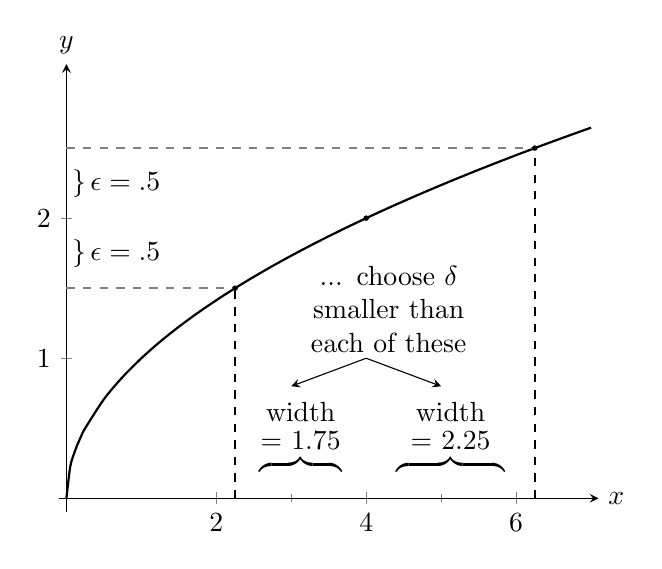
\begin{tikzpicture}[>=stealth]
    \begin{axis}[minor x tick num=1,axis y line=middle,axis x line=middle,ymin=-.1,ymax=3.1,xmin=-.1,xmax=7.1,xtick={2,4,6},ytick={1,2},name=myplot]
    \addplot [{\colorone},smooth,thick] coordinates {(0.,0.) (0.05,0.223607) (0.1,0.316228) (0.15,0.387298) (0.2,0.447214) (0.25,0.5) (0.5,0.707107) (0.75,0.866025) (1.,1.) (1.25,1.11803) (1.5,1.22474) (1.75,1.32288) (2.,1.41421) (2.25,1.5)(2.5,1.58114) (2.75,1.65831) (3.,1.73205) (3.25,1.80278)(3.5,1.87083) (3.75,1.93649) (4.,2.) (4.25,2.06155) (4.5,2.12132)(4.75,2.17945) (5.,2.23607) (5.25,2.29129) (5.5,2.34521) (5.75,2.39792) (6.,2.44949) (6.25,2.5)(6.5,2.54951) (6.75,2.59808) (7.,2.64575) 
    };
    \fill[black] (axis cs:4,2) circle (1pt);
    \draw[thin,dashed,gray,thick] (axis cs:0,1.5) -- (axis cs:2.25,1.5);
    \draw[thin,dashed,gray,thick] (axis cs:0,2.5) -- (axis cs:6.25,2.5);
    \draw[thin,dashed,{\colortwo},thick] (axis cs:2.25,0) -- (axis cs:2.25,1.5);
    \draw[thin,dashed,{\colortwo},thick] (axis cs:6.25,0) -- (axis cs:6.25,2.5);
    \draw (axis cs:-.1,1.75) node [right]{$\left.\rule{0pt}{7.5pt}\right\}\epsilon = .5$};
    \draw (axis cs:-.1,2.25) node [right]{$\left.\rule{0pt}{7.5pt}\right\}\epsilon = .5$};
    \fill[{\colortwo}] (axis cs:2.25,1.5) circle (1pt);
    \fill[{\colortwo}] (axis cs:6.25,2.5) circle (1pt);
    \draw (axis cs:3.125,.1) node [above,align=center,text width = 45pt] { width\\[-2pt] = 1.75\\[-3pt] $\overbrace{\rule{30pt}{0pt}}$};
    \draw (axis cs:5.125,.1) node [above,align=center,text width = 45pt] { width\\[-2pt] = 2.25\\[-3pt] $\overbrace{\rule{39pt}{0pt}}$};
    \draw (axis cs:4.3,1.35)	node [align=center,text width = 80pt] { ... choose $\delta$ smaller than each of these};
    \draw [->,thin] (axis cs:4,1) -- (axis cs:3,.8);
    \draw [->,thin] (axis cs:4,1) -- (axis cs:5,.8);
    \end{axis}
    %\fill[{\colortwo}] (1,1) circle (1pt);
    \node [right] at (myplot.right of origin) { $x$};
    \node [above] at (myplot.above origin) { $y$};
    \end{tikzpicture}
        \label{ }
        \caption{With $\epsilon=0.5$, we pick any $\delta < 1.75$.}    
    \end{subfigure} 
    \caption{ Illustrating the $\epsilon-\delta$ process. \label{fig:choose_e_d}}
\end{figure}

NOTE: The concept of a \dfont{one-sided limit} can also be made precise.

\begin{definition}{One-sided Limit}{onesided}
 Suppose that $f(x)$ is a function. We say that
$\ds \lim_{x\to a^-}f(x)=L$ if for every $\epsilon>0$ there is a $\delta >
0$ so that whenever $0 < a-x < \delta$, $|f(x)-L|<\epsilon$.  We say
that $\ds\lim_{x\to a^+}f(x)=L$ if for every $\epsilon>0$ there is a
$\delta > 0$ so that whenever $0 < x-a < \delta$, $|f(x)-L|<\epsilon$.
\end{definition}

%\mtable{.4}{Illustrating the $\epsilon-\delta$ process.}{fig:choose_e_d}{%
%%		\begin{tabular}{c} 
%		\myincludegraphics{figures/figLimitProof1a}\\
%		\myincludegraphics{figures/figLimitProof1b}\\
%		\noindent\parbox{200pt}{With $\epsilon=0.5$, we pick any $\delta < 1.75$.}
%%		\end{tabular}
%	}

		

Given the $y$ tolerance $\epsilon =0.5$, we have found an $x$ tolerance, $\delta \leq 1.75$, such that whenever $x$ is within $\delta$ units of 4, then $y$ is within $\epsilon$ units of 2.  That's what we were trying to find.\\
  
Let's try another value of $\epsilon$.\\

What if the $y$ tolerance is 0.01, i.e.,  $\epsilon =0.01$?  How close to 4 does $x$ have to be in order for $y$ to be within 0.01 units of 2 (or $1.99 < y < 2.01$)?  Again, we just square these values to get
$1.99^2 < x < 2.01^2$, or 
$$3.9601 < x < 4.0401.$$  
What is the desired $x$ tolerance?  In this case we must have $\delta \leq 0.0399$, which is the minimum distance from 4 of the two bounds given above.  %Note that in some sense, it looks like there are two tolerances (below 4 of 0.0399 units and above 4 of 0.0401 units).  However, we couldn't use the larger value of $0.0401$ for $\delta$ since then the interval for $x$ would be  $3.9599 < x < 4.0401$ resulting in $y$ values of $1.98995 < y < 2.01$ (which contains values NOT within 0.01 units of 2).\\

What we have so far: if $\epsilon =0.5$, then $\delta \leq 1.75$ and if $\epsilon = 0.01$, then $\delta \leq 0.0399$. A pattern is not easy to see, so we switch to general $\epsilon$ try to determine $\delta$ symbolically.  We start by assuming $y=\sqrt{x}$ is within $\epsilon$ units of 2:

\begin{eqnarray*}
|y - 2| < \epsilon &\\
-\epsilon < y - 2 < \epsilon& \qquad \textrm{(Definition of absolute value)}\\
-\epsilon < \sqrt{x} - 2 < \epsilon  &\qquad (y=\sqrt{x})\\
2 - \epsilon < \sqrt{x} < 2+ \epsilon &\qquad \textrm{ (Add 2)}\\
(2 - \epsilon)^2 < x < (2+ \epsilon) ^2 &\qquad \textrm{ (Square all)}\\
4 - 4\epsilon + \epsilon^2 < x < 4 + 4\epsilon + \epsilon^2 &\qquad \textrm{ (Expand)}\\
4 - (4\epsilon - \epsilon^2) < x < 4 + (4\epsilon + \epsilon^2). &\qquad \textrm{ (Rewrite in the desired form)}
\end{eqnarray*}

The ``desired form'' in the last step is ``$4-\textit{something} < x < 4 +\textit{something}$.''
Since we want this last interval to describe an $x$ tolerance around 4, we have that either $\delta \leq 4\epsilon - \epsilon^2$ or $\delta \leq 4\epsilon + \epsilon^2$, whichever is smaller: $$\delta \leq \min\{4\epsilon - \epsilon^2, 4\epsilon + \epsilon^2\}.$$  Since $\epsilon > 0$, the minimum is $\delta \leq 4\epsilon - \epsilon^2$.  That's the formula: given an $\epsilon$, set $\delta \leq 4\epsilon-\epsilon^2$. 

We can check this for our previous values.  If $\epsilon=0.5$, the formula gives
$\delta \leq 4(0.5) - (0.5)^2 = 1.75$ and when $\epsilon=0.01$, the formula gives $\delta \leq 4(0.01) - (0.01)^2 = 0.399$.
%\drawexampleline

So given any $\epsilon >0$, set $\delta \leq 4\epsilon - \epsilon^2$. Then if $|x-4|<\delta$ (and $x\neq 4$), then $|f(x) - 2| < \epsilon$,  satisfying the definition of the limit.  We have shown formally (and finally!) that $\displaystyle \lim_{x\rightarrow 4} \sqrt{x} = 2 $.
}
\end{solution}




%FOOTNOTE $**$: Actually, it is a pain, but this won't work if $\epsilon \ge 4$.  This shouldn't really occur since $\epsilon$ is supposed to be small, but it could happen.  In the cases where $\epsilon \ge 4$, just take $\delta = 1$ and you'll be fine.
The previous example was a little long in that we sampled a few specific cases of $\epsilon$ before handling the general case. Normally this is not done.  The previous example is also a bit unsatisfying in that $\sqrt{4}=2$; why work so hard to prove something so obvious? Many $\epsilon$-$\delta$ proofs are long and difficult to do. In this section, we will focus on examples where the answer is, frankly, obvious, because the non--obvious examples are even harder. In the next section we will learn some theorems that allow us to evaluate limits \textit{analytically}, that is, without using the $\epsilon$-$\delta$ definition.\\
%That is why theorems about limits are so useful! After doing a few more $\epsilon$--$\delta$ proofs, you will really appreciate the analytical ``short cuts'' found in the next section.\\

\begin{example}{Evaluating a limit using the definition}{ex_compute_lim2}{
Show that $\displaystyle \lim_{x\rightarrow 2} x^2 = 4$.}
\end{example}


\begin{solution}
{Let's do this example symbolically from the start.  Let $\epsilon > 0$ be given; we want $|y-4| < \epsilon$, i.e.,  $|x^2-4| < \epsilon$.  How do we find $\delta$ such that when $|x-2| < \delta$, we are guaranteed that $|x^2-4|<\epsilon$?% for some $\delta$ (in terms of $\epsilon$)?

This is a bit trickier than the previous example, but let's start by noticing that 
$|x^2-4| = |x-2|\cdot|x+2|$.  Consider:\\
\begin{equation} |x^2-4| < \epsilon \longrightarrow |x-2|\cdot|x+2| < \epsilon \longrightarrow |x-2| < \frac{\epsilon}{|x+2|}.\label{eq:limit1}\end{equation} 
Could we not set $\displaystyle \delta = \frac{\epsilon}{|x+2|}$?  

We are close to an answer, but the catch is that $\delta$ must be a \textit{constant} value (so it can't contain $x$).  There is a way to work around this, but we do have to make an assumption.  Remember that $\epsilon$ is supposed to be a small number, which implies that $\delta$ will also be a small value.  In particular, we can (probably) assume that $\delta < 1$.  If this is true, then $|x-2| < \delta$ would imply that $|x-2| < 1$, giving $1 < x < 3$.  

Now, back to the fraction $\displaystyle \frac{\epsilon}{|x+2|}$.  If $1<x<3$, then $3<x+2<5$ (add 2 to all terms in the inequality).  Taking reciprocals, we have 
\begin{align}
\frac15 <& \frac1{|x+2|} < \frac 13 & \text{which implies}\notag\\
\frac15 <& \frac1{|x+2|} & \text{which implies}\notag\\
\frac\epsilon5<&\frac{\epsilon}{|x+2|}.\label{eq:limit2}
\end{align}

%$\displaystyle \frac{1}{5}<\frac{1}{|x+2|}<\frac{1}{3}$ so that, in particular, 
%\begin{equation} \frac{\epsilon}{5}<\frac{\epsilon}{|x+2|}.\label{eq:limit2}\end{equation}  
This suggests that we set 
$\displaystyle \delta \leq \frac{\epsilon}{5}$. To see why, let consider what follows when we assume $|x-2|<\delta$:

\small
\begin{align*}
|x - 2| &< \delta &\\
|x - 2| &< \frac{\epsilon}{5}&  \text{\small(Our choice of $\delta$)}\\
|x - 2|\cdot|x + 2| &< |x + 2|\cdot\frac{\epsilon}{5}&  \text{\small(Multiply by $|x+2|$)}\\
|x^2 - 4|&< |x + 2|\cdot\frac{\epsilon}{5}&  \text{\small(Combine left side)}\\
|x^2 - 4|&< |x + 2|\cdot\frac{\epsilon}{5}< |x + 2|\cdot\frac{\epsilon}{|x+2|}=\epsilon &  
\text{\small(Using (\ref{eq:limit2}) as long as $\delta <1$)}
\end{align*}
\normalsize

We have arrived at $|x^2 - 4|<\epsilon$ as desired.  Note again, in order to make this happen we needed $\delta$ to first be less than 1.  That is a safe assumption; we want $\epsilon$ to be arbitrarily small, forcing $\delta$ to also be small. 

We have also picked $\delta$ to be smaller than ``necessary.'' We could get by with a slightly larger $\delta$, as shown in Figure \ref{fig:limit_eover5}. The dashed outer lines show the boundaries defined by our choice of $\epsilon$. The dotted inner lines show the boundaries defined by setting $\delta = \epsilon/5$. Note how these dotted lines are within the dashed lines. That is perfectly fine; by choosing $x$ within the dotted lines we are guaranteed that $f(x)$ will be within $\epsilon$ of 4.%If the value we eventually used for $\delta$, namely $\epsilon/5$, is not less than 1, this proof won't work.  For the final fix, we instead set $\delta$ to be the minimum of 1 and $\epsilon/5$. This way all calculations above work.  

\mfigure{.8}{Choosing $\delta = \epsilon/5$ in Example \ref{ex_compute_lim2}.}{fig:limit_eover5}{ %
\begin{tikzpicture}
\begin{axis}[axis y line=middle,axis x line=middle,ymin=2,ymax=6,xmin=1.3,xmax=3.3,xtick={2},ytick={4},name=myplot]
\addplot [{\colorone},smooth,thick] coordinates {((0.,0.) (0.25,0.0625) (0.5,0.25) (0.75,0.5625) (1.,1.) (1.25,1.5625)
(1.5,2.25) (1.75,3.0625) (2.,4.) (2.25,5.0625) (2.5,6.25)
(2.75,7.5625) (3.,9.) 
};
\fill[black] (axis cs:2,4) circle (1pt);
\draw[thin,dashed,thick,{\colortwo}] (axis cs:0,3) -- (axis cs:1.73,3);
\draw[thin,dashed,thick,{\colortwo}] (axis cs:0,5) -- (axis cs:2.24,5);
\draw[thin,dashed,thick,{\colortwo}] (axis cs:2.24,0) -- (axis cs:2.24,5);
\draw[thin,dashed,thick,{\colortwo}] (axis cs:1.73,0) -- (axis cs:1.73,3);
\draw[dotted,ultra thick,gray] (axis cs:2.2,0) -- (axis cs:2.2,4.84);
\draw[dotted,ultra thick,gray] (axis cs:1.8,0) -- (axis cs:1.8,3.24);
\draw (axis cs:-.1,4.5) node [right]{ $\left.\rule{0pt}{12pt}\right\}\epsilon$};
\draw (axis cs:2.1,2.15) node [above] { $\delta$};
\draw (axis cs:2.1,2.05) node [above,scale=.35] {$\overbrace{\phantom{..........}}$};
\draw (axis cs:2.3,4.5)  -- (axis cs: 3.2,4.5);
\draw (axis cs:2.3,4.3)  -- (axis cs: 2.5,4.3);
\draw (axis cs:2.75,4.7) node [align=center]{  length of $\epsilon$};
\draw (axis cs:2.75,3.9) node [align=center,text width=35pt]{ length of\\[-2pt] $\delta=\epsilon/5$};
\fill[{\colortwo}] (axis cs:1.73,3) circle (1pt);
\fill[{\colortwo}] (axis cs:2.24,5) circle (1pt);
\end{axis}
%\fill[{\colortwo}] (1,1) circle (1pt);
\node [right] at (myplot.right of origin) {  $x$};
\node [above] at (myplot.above origin) { $y$};
\end{tikzpicture}}

In summary, given $\epsilon > 0$, set $\delta=\leq\epsilon/5$.  Then $|x - 2| < \delta$ implies 
$|x^2 - 4|< \epsilon$ (i.e. $|y - 4|< \epsilon$) as desired.  This shows that $\displaystyle \lim_{x\rightarrow 2} x^2 = 4 $. Figure \ref{fig:limit_eover5} gives a visualization of this; by restricting $x$ to values within $\delta = \epsilon/5$ of 2, we see that $f(x)$ is within $\epsilon$ of $4$.
}
\end{solution}

It probably seems obvious that $\ds \lim_{x\to2}x^2=4$, and it is worth
examining more closely why it seems obvious. If we write $\ds x^2=x\cdot
x$, and ask what happens when $x$ approaches 2, we might say something
like, ``Well, the first $x$ approaches 2, and the second $x$
approaches 2, so the product must approach $2\cdot2$.'' In fact this is
pretty much right on the money, except for that word ``must.'' Is it
really true that if $x$ approaches $a$ and $y$ approaches $b$ then
$xy$ approaches $ab$? It is, but it is not really obvious, since $x$
and $y$ might be quite complicated. The good news is that we can see
that this is true once and for all, and then we don't have to worry
about it ever again. When we say that $x$ might be ``complicated'' we
really mean that in practice it might be a function. Here is then what
we want to know:

\begin{theorem}{Limit Product}{LimitProduct}
Suppose $\ds \lim_{x\to a} f(x)=L$ and $\ds \lim_{x\to a}g(x)=M$. Then
$\ds \lim_{x\to a} f(x)g(x) = LM$.
\end{theorem}

\begin{proof}
We must use the Precise Definition of a Limit to prove the Produce Law for Limits.
So given any $\epsilon$ we need to find a $\delta$ so that $0<|x-a|<\delta$ implies
$|f(x)g(x)-LM|<\epsilon$. What do we have to work with? We know that we can make 
$f(x)$ close to $L$ and $g(x)$ close to $M$, and we have to somehow connect these
facts to make $f(x)g(x)$ close to $LM$.

We use, as is often the case, a little algebraic trick:
\begin{align*}
|f(x)g(x)-LM|&=|f(x)g(x)-f(x)M+f(x)M-LM|	\\
&=|f(x)(g(x)-M)+(f(x)-L)M|	\\
&\leq |f(x)(g(x)-M)|+|(f(x)-L)M|	\\
&=|f(x)||g(x)-M|+|f(x)-L||M|.
\end{align*}

This is all straightforward except perhaps for the ``$\leq$''. That is an example
of the \emph{triangle inequality}, which says that if $a$ and $b$ are any real numbers
then $|a+b|\leq|a|+|b|$. If you look at a few examples, using positive and negative numbers
in various combinations for $a$ and $b$, you should quickly understand why this is true.
We will not prove it formally.

Suppose $\epsilon>0$. Since $\ds\lim_{x\to a} f(x)=L$, there is a value $\delta_1$
such that $0<|x-a|<\delta_1$ implies $\ds|f(x)-L|<\frac{\epsilon}{2(1+|M|)}$.
This means that $0<|x-a|<\delta_1$ implies $|f(x)-L||M|<|f(x)-L|(1+|M|)<\epsilon/2$.

Now we focus our attention on the other term in the inequality, $|f(x)||g(x)-M|$.
We can make $|g(x)-M|$ smaller than any fixed number by making $x$
close enough to $a$; unfortunately, $\epsilon/(2f(x))$ is not a fixed
number, since $x$ is a variable. Here we need another little trick,
just like the one we used in analyzing $x^2$. We can find a $\delta_2$
so that $|x-a|<\delta_2$ implies that $|f(x)-L|<1$, meaning that $L-1
< f(x) < L+1$. This means that $|f(x)|<N$, where $N$ is either $|L-1|$
or $|L+1|$, depending on whether $L$ is negative or positive. The
important point is that $N$ doesn't depend on $x$. Finally, we know that
there is a $\delta_3$ so that $0<|x-a|<\delta_3$ implies
$|g(x)-M|<\epsilon/(2N)$. Let $\delta$ be the smallest of $\delta_1$, $\delta_2$, and
$\delta_3$. Then $|x-a|<\delta$ implies that
$|f(x)-L|<\epsilon/(2(1+|M|))$, $|f(x)|<N$, and
$|g(x)-M|<\epsilon/(2N)$. Then 
\begin{align*}
|f(x)g(x)-LM|&\leq |f(x)||g(x)-M|+|f(x)-L||M|	\\
&< N\frac{\epsilon}{2N}+\frac{\epsilon}{2(1+|M|)}(1+|M|)	\\
&=\frac{\epsilon}{2}+\frac{\epsilon}{2}=\epsilon.
\end{align*}
This is just what we needed, so by the official definition,
$\ds \lim_{x\to a}f(x)g(x)=LM$.
\end{proof} 



Examples \ref{exa:ex_compute_lim1} and \ref{exa:ex_compute_lim2} determine $\delta$ by using logic that is difficult to recreate as one learns this topic. For instance, Equation \eqref{eq:limit2} is used based on the following facts:
	\begin{enumerate}
	\item		We want $\delta \leq \frac{\epsilon}{|x+2|}$. Since we cannot let $\delta$ vary according to $x$,
	\item		we notice that $|x+2|<5$ for the values we are interested in, so
	\item		$\frac{\epsilon}{5} < \frac{\epsilon}{|x+2|}$ and setting $\delta<\frac{\epsilon}{5}$ ensures that $\delta<\frac{\epsilon}{|x+2|}$.
	\end{enumerate}

The following theorem offers some inequalities that are useful when creating $\delta$--$\epsilon$ proofs.


\begin{theorem}{Power Function Inequalities}{power_ineq}
{Let $x>y>0$ and $n>1$. The following inequalities hold:
\begin{itemize}
\item		$\ds x^n+y^n < (x+y)^n$
\item		$\ds (x-y)^n < x^n - y^n$
\item		$\ds\sqrt[n]{x+y} < \sqrt[n]{x}+\sqrt[n]{y}$
\item		$\ds \sqrt[n]{x}-\sqrt[n]{y}<\sqrt[n]{x-y}$
\end{itemize}
}
\end{theorem}


%
%We revisit the limit found in Example \ref{ex_compute_lim2} to demonstrate the use of Theorem \ref{thm:power_ineq}.
%
%\example{ex_compute_lim2b}{Show that $\ds \lim_{x\to 2} x^2=4$ using Theorem \ref{thm:power_ineq}.}
%{We start the same as before; let $\epsilon >0$ be given. We want to find $\delta>0$ such that $|x^2-4|<\epsilon$ whenever $|x-2|<\delta$. Consider the following inequalities:
%\begin{align*}
%|x^2-4|<\epsilon & \\
%-\epsilon < x^2-4 < \epsilon & \qquad \text{\small (Definition of abs. value)}\\
%4-\epsilon < x^2 < 4+\epsilon & \qquad \text{\small (add 4)}\\
%\sqrt{4-\epsilon} < x < \sqrt{4+\epsilon} & \qquad \text{\small (Take square roots)}\\
%\sqrt{4}-\sqrt{\epsilon} < \sqrt{4-\epsilon} < x < \sqrt{4+\epsilon}< \sqrt{4}+\sqrt{\epsilon} & \qquad \text{\small (apply Theorem \ref{thm:power_ineq})}\\
%2-\sqrt{\epsilon} < x < 2 + \sqrt{\epsilon} & \text{\small (Simplify)}
%\end{align*}
%This implies that when $x$ is within $\sqrt{\epsilon}$ of $2$, $x^2$ will be within $\epsilon$ of $4$. Thus set $\delta = \sqrt{\epsilon}$. We can now start with $|x-2|<\delta$ and reverse the above steps:
%\begin{align*}
%|x-2| < \delta & \\
%-\delta < x-2 < \delta & \qquad \text{\small (Definition of abs. value)}\\
%2-\delta < x < 2+ \delta & \\
%2-\sqrt{\epsilon} < x < 2+\sqrt{\epsilon} & \\
%\end{align*}
%}

Make note of the general pattern exhibited in these last two examples. In some sense, each starts out ``backwards.'' That is, while we want to
\begin{enumerate}
	\item start with $|x-c|<\delta$ and conclude that
	\item $|f(x)-L|<\epsilon$,
\end{enumerate}
we actually start by assuming 
\begin{enumerate}
	\item $|f(x)-L|<\epsilon$, then perform some algebraic manipulations to give an inequality of the form
	\item $|x-c|<$ \textit{something}.
\end{enumerate} 
%then perform some algebraic manipulations to transform that inequality into an inequality where the ``less than'' side is $|x-c|$. 
When we have properly done this, the \textit{something} on the ``greater than'' side of the inequality becomes our $\delta$. We can refer to this as the ``scratch--work'' phase of our proof. Once we have $\delta$, we can formally start with $|x-c|<\delta$ and use algebraic manipulations to conclude that $|f(x)-L|<\epsilon$, usually by using the same steps of our ``scratch--work'' in reverse order.

We highlight this process in the following example.\\


\begin{example}{Evaluating a limit using the definition}{ex_compute_lim4}
{Prove that $\ds \lim_{x\rightarrow 1}x^3-2x = -1$.}
\end{example}


\begin{solution}
{We start our scratch--work by considering $|f(x) - (-1)| < \epsilon$:
\begin{align}
|f(x)-(-1)| &< \epsilon \notag\\
|x^3-2x + 1|&< \epsilon & \text{(Now factor)}\notag\\
|(x-1)(x^2+x-1)|&< \epsilon \notag\\
|x-1| &<\frac{\epsilon}{|x^2+x-1|}.\label{eq:lim4}
\end{align}
We are at the phase of saying that $|x-1|<$ \textit{something}, where \textit{something}$=\epsilon/|x^2+x-1|$. We want to turn that \textit{something} into $\delta$.

Since $x$ is approaching 1, we are safe to assume that $x$ is between 0 and 2. So
\begin{align*}
0&< x<2  & \\
0&< x^2<4.&\text{(squared each term)}\\
\intertext{Since $0<x<2$, we can add $0$, $x$ and $2$, respectively, to each part of the inequality and maintain the inequality.}
0&< x^2+x<6 &\\
-1&< x^2+x-1<5.&\text{(subtracted 1 from each part)}
\end{align*}

In Equation \eqref{eq:lim4}, we wanted $|x-1|<\epsilon/|x^2+x-1|$. The above shows that given any $x$ in $[0,2]$, we know that 
\begin{align}
x^2+x-1 &< 5 &\text{which implies that}\notag\\
\frac15 &< \frac{1}{x^2+x-1} &\text{which implies that}\notag\\
\frac{\epsilon}5 &< \frac{\epsilon}{x^2+x-1}.\label{eq:lim4b}
\end{align}
 So we set $\delta \leq \epsilon/5$. This ends our scratch--work, and we begin the formal proof (which also helps us understand why this was a good choice of $\delta$).

Given $\epsilon$, let $\delta \leq \epsilon/5$. We want to show that when $|x-1|<\delta$, then $|(x^3-2x)-(-1)|<\epsilon$. We start with $|x-1|<\delta$:
\begin{align*}
|x-1| &< \delta \\
|x-1| &< \frac{\epsilon}5\\
|x-1| &< \frac\epsilon5 < \frac{\epsilon}{|x^2+x-1|} & \text{(for $x$ near 1, from Equation \eqref{eq:lim4b})}\\
|x-1|\cdot |x^2+x-1| &< \epsilon\\
|x^3-2x+1| &< \epsilon\\
|(x^3-2x)-(-1)| &<\epsilon,
\end{align*}
which is what we wanted to show. Thus $\ds \lim_{x\to 1}x^3-2x = -1$.
}
\end{solution}



%
We illustrate evaluating limits once more.\\


\begin{example}{Evaluating a limit using the definition}{ex_compute_lim3}
{Prove that $\displaystyle \lim_{x\rightarrow 0} e^x = 1 $.}
\end{example}


\begin{solution}
{Symbolically, we want to take the equation $|e^x - 1| < \epsilon$ and unravel it to the form $|x-0| < \delta$.  Here is our scratch--work:
\begin{eqnarray*}
|e^x - 1| < \epsilon&\\
-\epsilon < e^x - 1 < \epsilon& \qquad \textrm{(Definition of absolute value)}\\
1-\epsilon < e^x < 1+\epsilon & \qquad \textrm{(Add 1)}\\
\ln(1-\epsilon) < x < \ln(1+\epsilon) & \qquad \textrm{(Take natural logs)}\\
\end{eqnarray*}
Making the safe assumption that $\epsilon<1$ ensures the last inequality is valid (i.e., so that $\ln (1-\epsilon)$ is defined). We can then set $\delta$ to be the minimum of $|\ln(1-\epsilon)|$ and $\ln(1+\epsilon)$; i.e.,  %  Well, there is a catch.  The value of $\epsilon$ is supposed to be small, but if it happens that $\epsilon \ge 1$, then $\ln(1-\epsilon)$ would be undefined!  The way to work around this is to simply define a new epsilon that is guaranteed to be smaller than the original epsilon \textit{and} less than 1 (let's say less than 1/2 just to be on the safe side).  Let's call this new value $\epsilon_1$ and define it to be $\epsilon_1 = \min\{\epsilon, 1/2\}$.  Then we can use the calculations above to define 
$$\delta = \min\{|\ln(1-\epsilon)|, \ln(1+\epsilon)\} = \ln(1+\epsilon).$$  
{\textbf{Note:} Recall $\ln 1= 0$ and $\ln x<0$ when $0<x<1$. So $\ln (1-\epsilon) <0$, hence we consider its absolute value.}

Now, we work through the actual the proof:


\begin{align*}
|x - 0|&<\delta\\
-\delta &< x < \delta &  \textrm{(Definition of absolute value)}\\
-\ln(1+\epsilon) &< x < \ln(1+\epsilon). &\\  
\ln(1-\epsilon) &< x < \ln(1+\epsilon). & \text{(since $\ln(1-\epsilon) < -\ln(1+\epsilon)$)}\\ 
\intertext{The above line is true by our choice of $\delta$ and by the fact that since $|\ln(1-\epsilon)|>\ln(1+\epsilon)$ and $\ln(1-\epsilon)<0$, we know $\ln(1-\epsilon) < -\ln(1+\epsilon )$.} %\textrm{(By our choice of}\; \delta)\\
1-\epsilon &< e^x < 1+\epsilon &  \textrm{(Exponentiate)}\\
-\epsilon &< e^x - 1 < \epsilon &  \textrm{(Subtract 1)}\\
%-\epsilon < e^x - 1 < \epsilon & \qquad \textrm{(Since}\; \epsilon_1 \le \epsilon)\\
\end{align*}

In summary, given $\epsilon > 0$, let $\delta = \ln(1+\epsilon)$. Then $|x - 0| < \delta$ implies $|e^x - 1|< \epsilon$ as desired.  We have shown that $\displaystyle \lim_{x\rightarrow 0} e^x = 1 $.
}
\end{solution}




We note that we could actually show that $\lim_{x\rightarrow c} e^x = e^c $ for any constant $c$.  We do this by factoring out $e^c$ from both sides, leaving us to show $\lim_{x\rightarrow c} e^{x-c} = 1 $ instead.  By using the substitution $u=x-c$, this reduces to showing $\lim_{u\rightarrow 0} e^u = 1 $ which we just did in the last example.  As an added benefit, this shows that in fact the function $f(x)=e^x$ is \textit{continuous} at all values of $x$, an important concept we will define in Section \ref{sec:Continuity}.\\

This formal definition of the limit is not an easy concept grasp. Our examples are actually ``easy'' examples, using ``simple'' functions like polynomials, square--roots and exponentials. It is very difficult to prove, using the techniques given above, that $\ds \lim_{x\to 0}(\sin x)/x = 1$, as we approximated in the previous section.

There is hope. The next section shows how one can evaluate complicated limits using certain basic limits as building blocks. While limits are an incredibly important part of calculus (and hence much of higher mathematics), rarely are limits evaluated using the definition. Rather, the techniques of the following section are employed.

\clearpage





%%%%%%%%%%%%%%%%%%%%%%%%%%%%%%%%%%%%%%%%%%%%
\Opensolutionfile{solutions}[ex]
\section*{Exercises for Section \ref{sec:LimitsFormal}}

\begin{enumialphparenastyle}


% % % % % % % % % % %
\begin{ex}
\begin{enumerate}
\item {What is wrong with the following ``definition'' of a limit?
	\begin{quote}
``The limit of $f(x)$, as $x$ approaches $a$, is $K$'' means that given any $\delta>0$ there exists $\epsilon>0$ such that whenever $|f(x)-K|< \epsilon$, we have $|x-a|<\delta$.
	\end{quote}
}

\item {Which is given first in establishing a limit, the $x$--tolerance or the $y$--tolerance?}

\item {T/F: $\epsilon$ must always be positive.}

\item {T/F: $\delta$ must always be positive.}
\end{enumerate}

\begin{sol}
\begin{enumerate}
\item {$\epsilon$ should be given first, and the restriction 	$|x-a|<\delta$ implies $|f(x)-K|< \epsilon$, not the other way around.}
\item {The $y$--tolerance.}
\item {T}
\item 
{T}
\end{enumerate}
\end{sol}

\end{ex}
% % % % % % % % % % % %
% % % % % % % % % % %
\begin{ex}
Prove the given limit using an $\epsilon - \delta$ proof.
\begin{enumerate}

\item {$\displaystyle \lim_{x\to 2} 5 = 5$}

\item {$\displaystyle \lim_{x\to 5} 3-x = -2$}

\item {$\displaystyle \lim_{x\to 3} x^2-3 = 6$}

\item {$\displaystyle \lim_{x\to 2} x^3-1 = 7$}
\item {$\displaystyle \lim_{x\to 0} e^{2x}-1 = 0$}

\item {$\displaystyle \lim_{x\to 0} \sin x= 0$ (Hint: use the fact that $|\sin x| \leq |x|$, with equality only when $x=0$.)}
\item {$\displaystyle \lim_{x\to 4} x^2+x-5 = 15$}

\end{enumerate}

\begin{sol}
\begin{enumerate}
\item {Let $\epsilon >0$ be given. We wish to find $\delta >0$ such that when $|x-2|<\delta$, $|f(x)-5|<\epsilon$. However, since $f(x)=5$, a constant function, the latter inequality is simply $|5-5|<\epsilon$, which is always true. Thus we can choose any $\delta$ we like; we arbitrarily choose $\delta =\epsilon$. 
}
\item {Let $\epsilon >0$ be given. We wish to find $\delta >0$ such that when $|x-5|<\delta$, $|f(x)-(-2)|<\epsilon$. 

Consider $|f(x)-(-2)|<\epsilon$:
\begin{gather*}
|f(x) + 2 | < \epsilon \\
|(3-x) + 2 |<\epsilon \\
| 5-x | < \epsilon \\
-\epsilon < 5-x < \epsilon \\
-\epsilon < x-5 < \epsilon. \\
\end{gather*}
This implies we can let $\delta =\epsilon$. Then:
\begin{gather*}
|x-5|<\delta \\
-\delta < x-5 < \delta\\
-\epsilon < x-5 < \epsilon\\
-\epsilon < (x-3)-2 < \epsilon \\
-\epsilon < (-x+3)-(-2) < \epsilon \\
|3-x - (-2)| < \epsilon,
\end{gather*}
which is what we wanted to prove.
}

\item {Let $\epsilon >0$ be given. We wish to find $\delta >0$ such that when $|x-3|<\delta$, $|f(x)-6|<\epsilon$. 

Consider $|f(x)-6|<\epsilon$, keeping in  mind we want to make a statement about $|x-3|$:
\begin{gather*}
|f(x) -6 | < \epsilon \\
|x^2-3 -6 |<\epsilon \\
| x^2-9 | < \epsilon \\
| x-3 |\cdot|x+3| < \epsilon \\
| x-3 | < \epsilon/|x+3| \\
\end{gather*}
Since $x$ is near 3, we can safely assume that, for instance, $2<x<4$. Thus
\begin{gather*}
2+3<x+3<4+3 \\
5 < x+3 < 7 \\
\frac{1}{7} < \frac{1}{x+3} < \frac{1}{5} \\
\frac{\epsilon}{7} < \frac{\epsilon}{x+3} < \frac{\epsilon}{5} \\
\end{gather*}
Let $\delta =\frac{\epsilon}{7}$. Then:
\begin{gather*}
|x-3|<\delta \\
|x-3| < \frac{\epsilon}7\\
|x-3| < \frac{\epsilon}{x+3}\\
|x-3|\cdot|x+3| < \frac{\epsilon}{x+3}\cdot|x+3|\\
\end{gather*}
Assuming $x$ is near 3, $x+3$ is positive and we can drop the absolute value signs on the right.
\begin{gather*}
|x-3|\cdot|x+3| < \frac{\epsilon}{x+3}\cdot(x+3)\\
|x^2-9| < \epsilon\\
|(x^2-3) - 6| < \epsilon,
\end{gather*}
which is what we wanted to prove.
}
\item 
{Let $\epsilon >0$ be given. We wish to find $\delta >0$ such that when $|x-2|<\delta$, $|f(x)-7|<\epsilon$. 

Consider $|f(x)-7|<\epsilon$, keeping in  mind we want to make a statement about $|x-2|$:
\begin{gather*}
|f(x) -7 | < \epsilon \\
|x^3-1 -7 |<\epsilon \\
| x^3-8 | < \epsilon \\
| x-2 |\cdot|x^2+2x+4| < \epsilon \\
| x-3 | < \epsilon/|x^2+2x+4| \\
\end{gather*}
Since $x$ is near 2, we can safely assume that, for instance, $1<x<3$. Thus
\begin{gather*}
1^2+2\cdot1+4<x^2+2x+4<3^2+2\cdot3+4 \\
7 < x^2+2x+4 < 19 \\
\frac{1}{19} < \frac{1}{x^2+2x+4} < \frac{1}{7} \\
\frac{\epsilon}{19} < \frac{\epsilon}{x^2+2x+4} < \frac{\epsilon}{7} \\
\end{gather*}
Let $\delta =\frac{\epsilon}{19}$. Then:
\begin{gather*}
|x-2|<\delta \\
|x-2| < \frac{\epsilon}{19}\\
|x-2| < \frac{\epsilon}{x^2+2x+4}\\
|x-2|\cdot|x^2+2x+4| < \frac{\epsilon}{x^2+2x+4}\cdot|x^2+2x+4|\\
\end{gather*}
Assuming $x$ is near 2, $x^2+2x+4$ is positive and we can drop the absolute value signs on the right.
\begin{gather*}
|x-2|\cdot|x^2+2x+4| < \frac{\epsilon}{x^2+2x+4}\cdot(x^2+2x+4)\\
|x^3-8| < \epsilon\\
|(x^3-1) - 7| < \epsilon,
\end{gather*}
which is what we wanted to prove.
}
\item {Let $\epsilon >0$ be given. We wish to find $\delta >0$ such that when $|x-0|<\delta$, $|f(x)-0|<\epsilon$. 

Consider $|f(x)-0|<\epsilon$, keeping in  mind we want to make a statement about $|x-0|$ (i.e., $|x|$):
\begin{gather*}
|f(x) -0 | < \epsilon \\
|e^{2x}-1 |<\epsilon \\
-\epsilon< e^{2x}-1 < \epsilon \\
1-\epsilon< e^{2x} < 1+\epsilon \\
\ln (1-\epsilon) < 2x < \ln (1+\epsilon) \\
\frac{\ln (1-\epsilon)}{2} < x < \frac{\ln (1+\epsilon)}{2} \\
\end{gather*}
Let $\delta = \min\left\{\left|\frac{\ln(1-\epsilon)}{2}\right|,\frac{\ln(1+\epsilon)}{2}\right\}=\frac{\ln(1+\epsilon)}{2}.$

Thus:
\begin{gather*}
|x| < \delta \\
%|x| < \min\left\{\left|\frac{\ln(1-\epsilon)}{2}\right|,\left|\frac{\ln(1+\epsilon)}{2}\right|\right\} \\
|x| <\frac{\ln(1+\epsilon)}{2}<\left|\frac{\ln(1-\epsilon)}{2}\right| \\
\frac{\ln(1-\epsilon)}{2} < x < \frac{\ln(1+\epsilon)}{2}\\
\ln(1-\epsilon)< 2x < \ln(1+\epsilon)\\
1-\epsilon < e^{2x} < 1+\epsilon\\
-\epsilon < e^{2x}-1 < \epsilon\\
|e^{2x}-1-(0)| < \epsilon,
\end{gather*}
which is what we wanted to prove.
}
\item 
{Let $\epsilon >0$ be given. We wish to find $\delta >0$ such that when $|x-0|<\delta$, $|f(x)-0|<\epsilon$. In simpler terms, we want to show that when $|x|<\delta$, $|\sin x| < \epsilon$. 

Set $\delta = \epsilon$. We start with assuming that $|x|<\delta$. Using the hint, we have that $|\sin x | < |x| < \delta = \epsilon$. Hence if $|x|<\delta$, we know immediately that $|\sin x| < \epsilon$.
}
\item {Let $\epsilon >0$ be given. We wish to find $\delta >0$ such that when $|x-4|<\delta$, $|f(x)-15|<\epsilon$. 

Consider $|f(x)-15|<\epsilon$, keeping in  mind we want to make a statement about $|x-4|$:
\begin{gather*}
|f(x) -15 | < \epsilon \\
|x^2+x-5 -15 |<\epsilon \\
| x^2+x-20 | < \epsilon \\
| x-4 |\cdot|x+5| < \epsilon \\
| x-4 | < \epsilon/|x+5| \\
\end{gather*}
Since $x$ is near 4, we can safely assume that, for instance, $3<x<5$. Thus
\begin{gather*}
3+5<x+5<5+5 \\
8 < x+5 < 10 \\
\frac{1}{10} < \frac{1}{x+5} < \frac{1}{8} \\
\frac{\epsilon}{10} < \frac{\epsilon}{x+5} < \frac{\epsilon}{8} \\
\end{gather*}
Let $\delta =\frac{\epsilon}{10}$. Then:
\begin{gather*}
|x-4|<\delta \\
|x-4| < \frac{\epsilon}{10}\\
|x-4| < \frac{\epsilon}{x+5}\\
|x-4|\cdot|x+5| < \frac{\epsilon}{x+5}\cdot|x+5|\\
\end{gather*}
Assuming $x$ is near 4, $x+5$ is positive and we can drop the absolute value signs on the right.
\begin{gather*}
|x-4|\cdot|x+5| < \frac{\epsilon}{x+5}\cdot(x+5)\\
|x^2+x-20| < \epsilon\\
|(x^2+x-5) -15| < \epsilon,
\end{gather*}
which is what we wanted to prove.
}

\end{enumerate}
\end{sol}

\end{ex}
% % % % % % % % % % % %


\begin{ex}
Let $\epsilon$ be a small positive real number. How close to 2 must we hold $x$ in order to be sure that $3x+1$ lies within $\epsilon$ units of 7?
\end{ex}

\end{enumialphparenastyle}

\clearpage